% $Header: /cvsroot/latex-beamer/latex-beamer/solutions/generic-talks/generic-ornate-15min-45min.en.tex,v 1.5 2007/01/28 20:48:23 tantau Exp $

\documentclass[12pt]{beamer}
%\documentclass[12pt,handout]{beamer}

% This file is a solution template for:

% - Giving a talk on some subject.
% - The talk is between 15min and 45min long.
% - Style is ornate.



% Copyright 2004 by Till Tantau <tantau@users.sourceforge.net>.
%
% In principle, this file can be redistributed and/or modified under
% the terms of the GNU Public License, version 2.
%
% However, this file is supposed to be a template to be modified
% for your own needs. For this reason, if you use this file as a
% template and not specifically distribute it as part of a another
% package/program, I grant the extra permission to freely copy and
% modify this file as you see fit and even to delete this copyright
% notice.


\mode<presentation>
{
  \usetheme{default}
  % or ...

  \setbeamercovered{transparent}
  % or whatever (possibly just delete it)
}
\setbeamertemplate{navigation symbols}{}%remove navigation symbols


\usepackage[english]{babel}
% or whatever

\usepackage[latin1]{inputenc}
% or whatever

\usepackage{times}
\usepackage{sansmathfonts}
\usepackage[T1]{fontenc}
% Or whatever. Note that the encoding and the font should match. If T1
% does not look nice, try deleting the line with the fontenc.


\title%[Short Paper Title] % (optional, use only with long paper titles)
{}

\subtitle
{} % (optional)

\author%[Author, Another] (optional, use only with lots of authors)
{Ben Holder}%{F.~Author\inst{1} \and S.~Another\inst{2}}
% - Use the \inst{?} command only if the authors have different
%   affiliation.

%\institute[Universities of Somewhere and Elsewhere] % (optional, but mostly needed)
%{
%  \inst{1}%
%  Department of Computer Science\\
%  University of Somewhere
%  \and
%  \inst{2}%
%  Department of Theoretical Philosophy\\
%  University of Elsewhere}
%% - Use the \inst command only if there are several affiliations.
%% - Keep it simple, no one is interested in your street address.

\date%[Short Occasion] % (optional)
{}

\subject{Talks}
% This is only inserted into the PDF information catalog. Can be left
% out.



% If you have a file called "university-logo-filename.xxx", where xxx
% is a graphic format that can be processed by latex or pdflatex,
% resp., then you can add a logo as follows:

% \pgfdeclareimage[height=0.5cm]{university-logo}{university-logo-filename}
% \logo{\pgfuseimage{university-logo}}



% Delete this, if you do not want the table of contents to pop up at
% the beginning of each subsection:
%\AtBeginSubsection[]
%{
%  \begin{frame}<beamer>{Outline}
%    \tableofcontents[currentsection,currentsubsection]
%  \end{frame}
%}


% If you wish to uncover everything in a step-wise fashion, uncomment
% the following command:

%\beamerdefaultoverlayspecification{<+->}

\usepackage{enumerate}
\usepackage{amsmath}
\usepackage{amssymb}
\usepackage[amssymb]{SIunits}
\usepackage{url}
\usepackage{hyperref}
\usepackage[normalem]{ulem}


\setbeamercovered{invisible}

\hypersetup{
    colorlinks=true,     % false: boxed links; true: colored links
    linkcolor=red,       % color of internal links
    citecolor=blue,      % color of links to bibliography
    filecolor=blue,      % color of file links
    urlcolor=blue        % color of external links
}


\begin{document}

%\begin{frame}
%  \titlepage
%\end{frame}

%%%%%%%%%%%%%%%%%%%%%%%%%%%%%%%%%%%%%%
\begin{frame}{Announcements}
	%
	\begin{itemize}
	\addtolength{\itemsep}{0.5\baselineskip}
	\item Any questions/issues?
	\item \underline{Schedule}:
		%
		\begin{itemize}
		\item[]{\bf Today (Follow-up)}: Discussion Q2 (estimating solar constant)
		\item[]{\bf Today (New)}: Atmosphere and Greenhouse Effect (week 2) --- Electricity and Magnetism, and Quantum Mechanics!
		\item[]{\bf Tomorrow (Lab)}: Cooling by radiation, interaction of light and molecules
		\item[]{\bf Thursday (Discussion)}: Understanding molecule-light interactions, spectral lines of atmosphere
		\item Next Week: Water and Phase transitions (Part I)
		\end{itemize}
		%
	\end{itemize}

\end{frame}
%%%%%%%%%%%%%%%%%%%%%%%%%%%%%%%%%%%%%%
\begin{frame}{Today's Reading Quiz (3 min)}


	
\vspace{1cm}

On your own sheet of paper\ldots

\vspace{0.5cm}

{\bf What makes a particular gas a greenhouse gas?  Give two examples of greenhouse gases and two examples of atmospheric gases that are not greenhouse gases.}

\vspace{0.5cm}

Turn in to Blackboard as scanned pdf (or image is fine).

\end{frame}
%%%%%%%%%%%%%%%%%%%%%%%%%%%%%%%%%%%%%%
\begin{frame}{Question 2 from Discussion}

\begin{center}
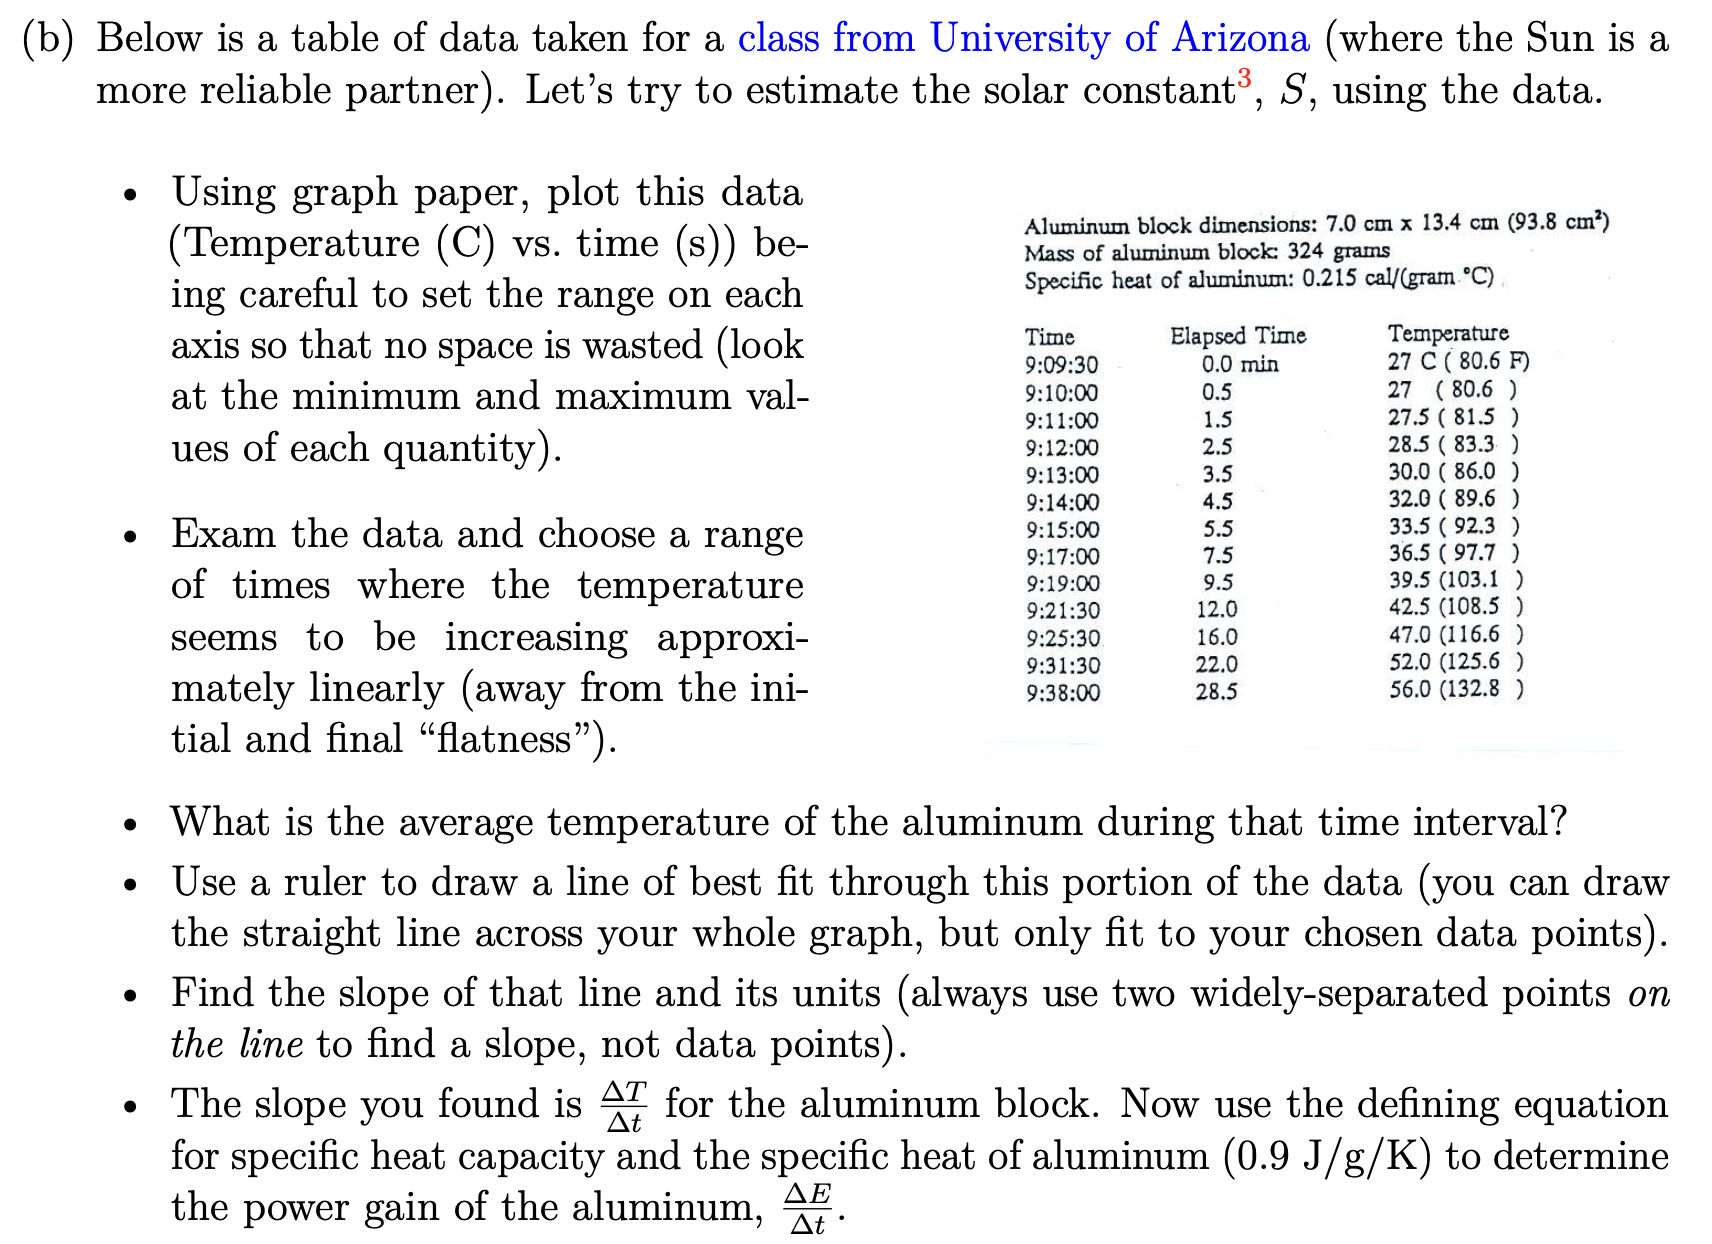
\includegraphics[width=0.7\textwidth]{images/disc05_Q2}
\end{center}

\end{frame}
%%%%%%%%%%%%%%%%%%%%%%%%%%%%%%%%%%%%%%
\begin{frame}{Question 2 from Discussion}



\end{frame}
%%%%%%%%%%%%%%%%%%%%%%%%%%%%%%%%%%%%%%
\begin{frame}{Charge and Electric Force}

\begin{itemize}
\item There are two types of electric charge: positive (held by protons) and negative (held by electrons). 
\item Atoms are neutral (same number of protons and electrons), but could become ionized (lose or gain electron) or shift their distribution of charge when bonding.
\item Like charges repel, opposite charges attract. (the {\em Coulomb Force})
\end{itemize}

\vspace{4cm}

\end{frame}
%%%%%%%%%%%%%%%%%%%%%%%%%%%%%%%%%%%%%%
\begin{frame}{Electric Field}

\begin{itemize}
\item Physicists don't like ``action at a distance'' so they use {\em fields} produced by charges (or masses: the gravitational field) to convey forces.
\item Positive charges have electric fields pointing away, negative have fields pointing towards.
\end{itemize}

\vspace{5cm}

\noindent {\small Force of electric field on charge: $\vec{F}_E = q \vec{E}$ (opp/same dir $q \lessgtr 0$)}
\end{frame}
%%%%%%%%%%%%%%%%%%%%%%%%%%%%%%%%%%%%%%
\begin{frame}{Electric Dipole}

\noindent A perfect dipole is two equal magnitude charges held apart at a distance $d$.  We write it as a vector $\vec{\mu}$ (Greek letter $\mu$)

\vspace{7cm}

\end{frame}
%%%%%%%%%%%%%%%%%%%%%%%%%%%%%%%%%%%%%%
\begin{frame}{Electromagnetic Wave and a dipole}



\vspace{7cm}


\end{frame}
%%%%%%%%%%%%%%%%%%%%%%%%%%%%%%%%%%%%%%
\begin{frame}{Interaction with EM field and a dipole (Classical)}


\vspace{7cm}


\end{frame}
%%%%%%%%%%%%%%%%%%%%%%%%%%%%%%%%%%%%%%
\begin{frame}{Interaction with EM field and a dipole (Quantum)}

\vspace{7cm}

\end{frame}
%%%%%%%%%%%%%%%%%%%%%%%%%%%%%%%%%%%%%%
\begin{frame}{Chemistry: Building Molecules}

\begin{itemize}
\item In Physics we construct the energy levels of a Hydrogen atom
\item The periodic table (Chemistry) fills in those energy levels with electrons (1 = H, 2 = He, 3 = Li, \ldots)
\item Recall the ``octet rule'' and Dot/Lewis diagrams
\end{itemize}

\vspace{7cm}

\end{frame}
%%%%%%%%%%%%%%%%%%%%%%%%%%%%%%%%%%%%%%
\begin{frame}{Chemistry: Building Molecules}

\begin{itemize}
\item Atmospheric gases that are not greenhouse, have no dipole.
\end{itemize}

\vspace{7cm}


\end{frame}
%%%%%%%%%%%%%%%%%%%%%%%%%%%%%%%%%%%%%%
\begin{frame}{Chemistry: Building Molecules}

\begin{itemize}
\item Atmospheric gases that are greenhouse, have the {\em possibilty} of a dipole.
\end{itemize}

\vspace{7cm}

\end{frame}
%%%%%%%%%%%%%%%%%%%%%%%%%%%%%%%%%%%%%%
\end{document}
